%! Author = filip
%! Date = 06/04/2025

% Preamble
\documentclass[11pt]{article}

% Packages
\usepackage{amsmath}
\usepackage{pifont}
\usepackage{graphicx}
\usepackage{listings}
\usepackage{xcolor}

\usepackage[margin=0.6in]{geometry}

\title{Genetic Optimisation Algorithms notes from AI course}
\author{Filip Dabkowski, Tomasz Kruczalak, ChatGPT}
\date{\today}


% Document
\begin{document}

    \maketitle

    \section[title]{Introduction}\label{sec:hello}

    \textbf{Genetic algorithm:}

    Search algorithms based on “natural evolution”.
    They are used to solve complex problems by evolving solutions through selection, crossover, and mutation.

    Previous algorithms began the search for the optimum in a single point, and intended to find a better solution for this single point.
    Gen-alg starts with $N$ starting points, and tries to improve \("\)worse\("\) points by making them more similar to \("\)better\("\) points.\\

    \textbf{Steps of GA}:
    \begin{itemize}
        \item \textbf{Initialization:} Starts with a population of $N$ potential solutions (chromosomes)
        \item \textbf{Evaluation:} Computes a fitness score for each chromosome (individual) based on a defined objective
        \item \textbf{Selection:} Choose the best individuals to create the next generation
        \item \textbf{Crossover (Recombination):} Combine selected individuals to produce new offspring
        \item \textbf{Mutation:} Introduce random changes to maintain genetic diversity
        \item \textbf{Replacement:} Form the new population and repeat the process\\
    \end{itemize}

    \textbf{Terms in genetic algorithms.} \textit{Maybe not the most important.}
    \begin{itemize}
        \item \textbf{phenotype:} physical expression or real-world behavior of a genotype.
        \item \textbf{genotype:} internal representation of a solution in a GA, usually represented as a binary string, list of numbers or other data structures.
        \item \textbf{chromosome:} complete set of genes representing a candidate solution in the population (e.g.:[101011])
        \item \textbf{allele:} specific value of a gene within a chromosome (e.g.: 1, 0)
        \item \textbf{locus:} gene position in chromosome.
        \item \textbf{fitness:} measure of how good a solution (chromosome) is, goal of GA is to maximize fitness.\\
    \end{itemize}

    \break

    \textbf{Basic genetic operators:}
    \begin{itemize}
        \item \textbf{Selection} (Reproduction)
        \item \textbf{Crossover} (Recombination)
        \item \textbf{Mutation}\\
    \end{itemize}

    \textbf{Selection (Reproduction):}
    \begin{itemize}
        \item Determines which individuals “pass their genes” to the next generation
        \item Higher fitness individuals have a better chance of being selected\\
    \end{itemize}

    \textbf{Crossover (Recombination):}
    \begin{itemize}
        \item Combines genes of two parents (individuals) to create offspring
        \item Mimics genetic recombination in nature
        \item \textbf{Common types:} Single-point, Multi-point, and Uniform crossover\\
    \end{itemize}

    \textbf{Mutation:}
    \begin{itemize}
        \item Randomly alters genes in an individual to maintain diversity
        \item Helps avoid local optima by introducing new traits
        \item \textbf{Types:} Bit Flip, Swap, Scramble, Gaussian mutation (for continuous values)\\
    \end{itemize}

    \textbf{Reproduction types:}
    \begin{itemize}
        \item \textbf{Roulette Wheel Selection:} chose individuals proportionally to the fitness value.
        \item \textbf{Rank-Based:} individuals are ranked based on fitness value, instead of using raw values.
        \item \textbf{Tournament:} multiple selection of the best individual from a randomly selected subpopulation.\\
    \end{itemize}

    \textbf{Actions related to genetic algorithm implementation:}
    \begin{itemize}
        \item Choice of coding method phenotype representation (solutions)
        \item Selection of genetic operators depending on the problem and the coding method used
        \item Selection of evolution parameters values
        \item Selection of fitness evaluation function
    \end{itemize}

    \break

    \textbf{Genetic Algorithm Schema:}
    \begin{figure}[h]
        \centering
        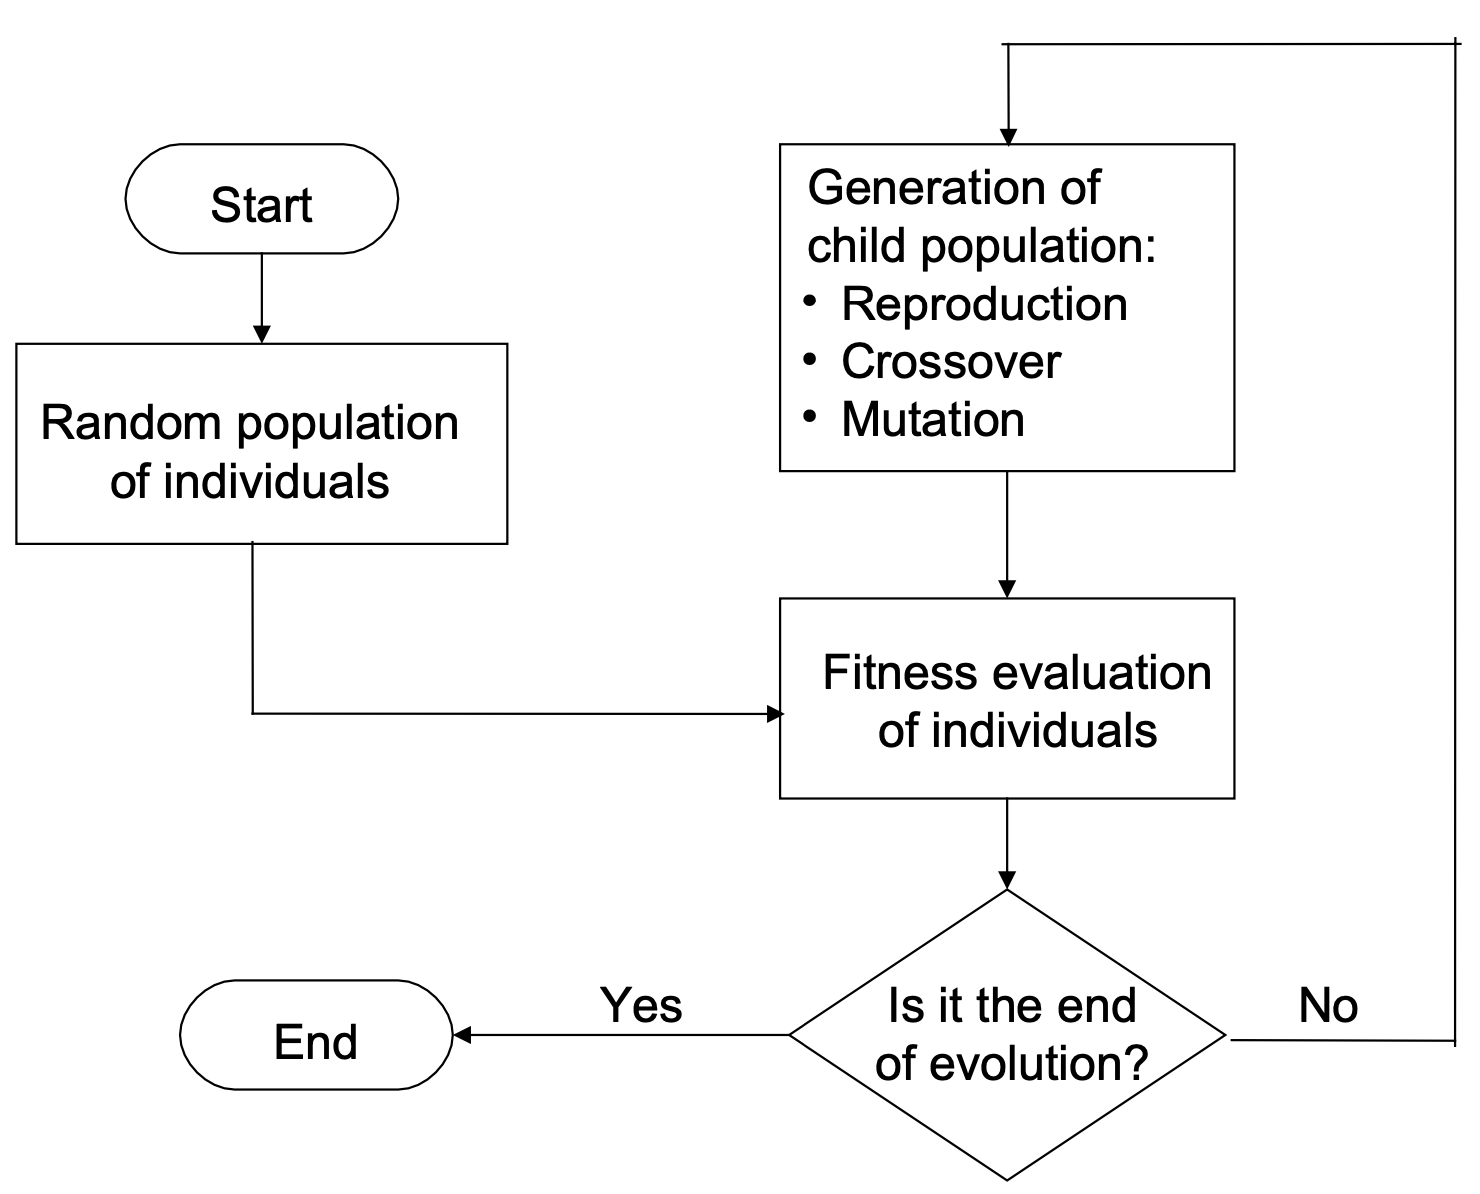
\includegraphics[width=0.5\textwidth]{../images/GA-LifeCycle}
        \caption{Life cycle of GA}\label{fig:image-GA-LifeCycle}
    \end{figure}


    \section{Implementation Details}\label{sec:implementation-details}

    \subsection{Roulette Selection}\label{subsec:roulette-reproduction}

    Lets use a simple example we have a chromosome $v = [x_1, x_2]$, and our fittness function:
    \begin{equation}
        f(v) = -(x_1 + x_2-5)^2 + 25
        \label{eq:fitness-f}
    \end{equation}
    \textit{The closer the sum of $x_1$ and $x_2$ is to $5$ the higher the fittnes. As the fittness should always be non-negative, lets say we only conder values in range [0, 5]}\\

    \textbf{Now the population with $N=4$ individuals is:}

    \begin{table}[h!]
        \centering
        \begin{tabular}{|l|c|c|}
            \hline
            \textbf{Individual} & \textbf{$v$} & \textbf{Fittness} \\
            \hline
            A                   & $[1, 2]$     & 21                \\
            B                   & $[1, 3]$     & 24                \\
            C                   & $[0, 0]$     & 0                 \\
            D                   & $[4, 4]$     & 16                \\
            \hline
        \end{tabular}
        \label{tab:roulette-table}
    \end{table}

    Now we determine the probability of being picked for reproduction, with Roulette the probability is a simple scaling calculation.
    As a population can be large and some individuals with a lot higher fitness may overwhelm the calculation, you may decide to assign some minimal probability.
    This can help in not being stuck in local minima, by allowing more exploration and ability to make not optimal decisions.

    \begin{equation}
        p(v) = \frac{f(v)}{\sum^N_{i=1} f(v_i)}
        \label{eq:roulette-p}
    \end{equation}

    \textit{Here $v$ is the individual, while $v_i$ means iterating over all individuals in the popualtion.}

    From here as we want to keep the population the same size, we draw $N$ individuals.
    There is a possibility of the same individual being picked for reproduction, whether it is allowed with mutation, or not, then the selection is run again.
    Two individuals picked in the selection, will be then handled by crossover and mutation.

    \subsection{Rank Selection}\label{subsec:rank-selection}

    Another method for selecting parents is based on ranks, rather than scaling the percentages based on raw fittness values.
    An advantage of this is individuals with much higher do not completely dominate the population, more stable than roulette, however it is slower to converge.\\

    \textbf{Equation for Linear Rank Selection}

    \begin{equation}
        p(x) = a + k\left( 1 - \frac{r(x)}{N} \right)
        \label{eq:linear-rank-select}
    \end{equation}
    Legent for variables:
    \begin{itemize}
        \item $p(x)$: probability for individual $x$
        \item $x$: single individual
        \item $r(x)$: rank of individual $x$ ($r = 1$: best individual, $r_{\max}$: worst individual)
        \item $N$: population size
        \item $a$: base selection probability
        \item $k$: scaling factor to ensure probability sums up to 1\\
    \end{itemize}

    \textbf{Equation for Exponential Rank Selection}

    \begin{equation}
        p(x) = a + k\left( N - r(x) \right)^b
        \label{eq:exponential-rank-select}
    \end{equation}
    Legent for additional variables:
    \begin{itemize}
        \item $b$ - \textbf{power exponent} controlling \textbf{selective pressure}
    \end{itemize}

    \textit{Note: There exist more formulas for example with selection pressure for linear rank selection, and so on.}

    Now continuing the example from above, lets calculate the probabilities using the simple Linear Rank Selection.

    \begin{table}[h!]
        \centering
        \begin{tabular}{|l|c|c|c|c|}
            \hline
            \textbf{Individual} & \textbf{$v$} & \textbf{Fittness} & \textbf{Rank} & \textbf{$p(v), k=\frac{2}{3}, a=0$} \\
            \hline
            A                   & $[1, 2]$     & 21                & 2             & 0.33                                \\
            B                   & $[1, 3]$     & 24                & 1             & 0.5                                 \\
            C                   & $[0, 0]$     & 0                 & 4             & 0                                   \\
            D                   & $[4, 4]$     & 16                & 3             & 0.17                                \\
            \hline
        \end{tabular}
        \label{tab:linear-rank}
    \end{table}


    \section{Crossover}\label{sec:crossover}
    Crossover is a stage in GAs when from two selected parents a new instance is created.\\

    \subsection{Single-Point Crossover (for vectors, and lists like structures)}\label{subsec:single-point-crossover}
    Randomly picking a split point in $\left[ 1, d \right]$, where $d$ is number of dimension of some vector $x$.
    Then taking the first part from the beginning of a vector to a split point from $x_1$ and from split point to the end form $x_2$
    For loger gene sequences you can use Multi-Point Crossover where you define multiple points to divide the parents.
    \begin{verbatim}
def cross_single_point(x_1, x_2):
    split_point = randint(0, len(x))
    x_new = x_1[:split_point] + x_2[split_point:]
    \end{verbatim}
    
    \subsection{Average Crossover (when genes are continuous)}\label{subsec:average-crossover}
    To create a new individual we take a simple average of its parents.
    \begin{verbatim}
def cross_average(x_1, x_2):
    x_new = (x_1 + x_2) / 2
    \end{verbatim}
    
    \subsection{Uniform Crossover}\label{subsec:uniform-crossover}
    To create a new individual, for each gene (\textit{element in vector}) choose random from parent genes.
    \begin{verbatim}
def cross_uniform(x_1, x_2):
    x_new = [
        random.choice(x_1[0], x_2[0]),
        random.choice(x_1[1], x_2[1])
    ]
    \end{verbatim}
    
    \subsection{Heuristic Crossover (when genes are continuous)}\label{subsec:heuristic-crossover}
    This can be thought about as an extension of average crossover, however with preference towards the better (judged by fitness) parent.
    \textit{Here alpha is random number from 0 to 1, and $x_1$ is the parent with higher fitness.}
    \begin{verbatim}
def cross_heuristic(x_1, x_2):
    alpha = random()
    x_new = x_1 + alpha * (x_1 - x_2)
    \end{verbatim}
    
    \section{Mutation}\label{sec:mutation}
    Mutation is the last step in creating new population, after crossover when new individuals are created, there is a chance to add randomness to newly created individual.
    This help with exploration and finding new areas of possible solutions.
    
    \subsection{Gaussian Mutation (when genes are continuous)}\label{subsec:gaussian-mutation}
    Adding a small noise to a single gene, this method is great for fine-tuning.
    \begin{verbatim}
def mutate_gaussian(gene):
    gene_new = gene + random.gauss(0, 0.1)
    \end{verbatim}
    
    \subsection{Creep Mutation}\label{subsec:creep-mutation}
    Similar to Gauss Mutation however bounded to integers, making it more deterministic and suitable for discrete variables.
    \begin{verbatim}
def mutate_creep(gene):
    gene_new = gene + random.choice(-1, 1)
    \end{verbatim}

    \subsection{Uniform Mutation (requires knowledge of value range of the gene)}\label{subsec:uniform-mutation}
    Here you replace given gene with a completely random value from the range of this gene.
    \begin{verbatim}
def mutate_gaussian(range_min, range_max):
    gene_new = randint(range_min, range_max)
    \end{verbatim}

    \section{Additional Info}\label{sec:additional-info}
    
    \subsection{Important terms}\label{subsec:important-terms}
    
    \begin{itemize}
        \item \textbf{Selective Pressure}: action of increasing probability of being picked in the next population with respect to fitness.
        \item \textbf{Elitism}: the best individuals in the population go to the next generation without any change 
    \end{itemize}
    
    \subsection{Assumptions}\label{subsec:assumptions}
    
    \begin{itemize}
        \item Fitness value should be non-negative and for better performing individuals higher.
        \item Probabilities of picking an individual during, reproduction selection should be between $[0, 1]$ and sum up to $1$.
    \end{itemize}
    
    \subsection{Notes}\label{subsec:notes}
    
    As usual the best solution for picking the correct reproduction selection, cross-over method and mutation is problem dependant.
    
    As well as picking the best hyperparameter values.

\end{document}
